\chapter{Introduction}
This project concerns an energy system for handling energy production and consumption, the project is divided into smaller parts for several teams, where this report is concerning the energy hub, which is handling inputs from other devices that produces or consumes energy. The project is made on 3rd and 4th semester in the Electronic design engineering program at AU-Herning, where this document is primarily on the realisation of the project.
\paragraph{Reading guidelines}
This project is split into a technical process documentation and a non-technical documentation, as shown in the figure below. The non-technical document is describing the project and the final product, and referring to the working process and the documentation in the technical process document. Both the technical process documentation and the non-technical documentation includes common appendix with extra documentation and project parts.
\begin{figure}[H]
	\begin{centering}
		 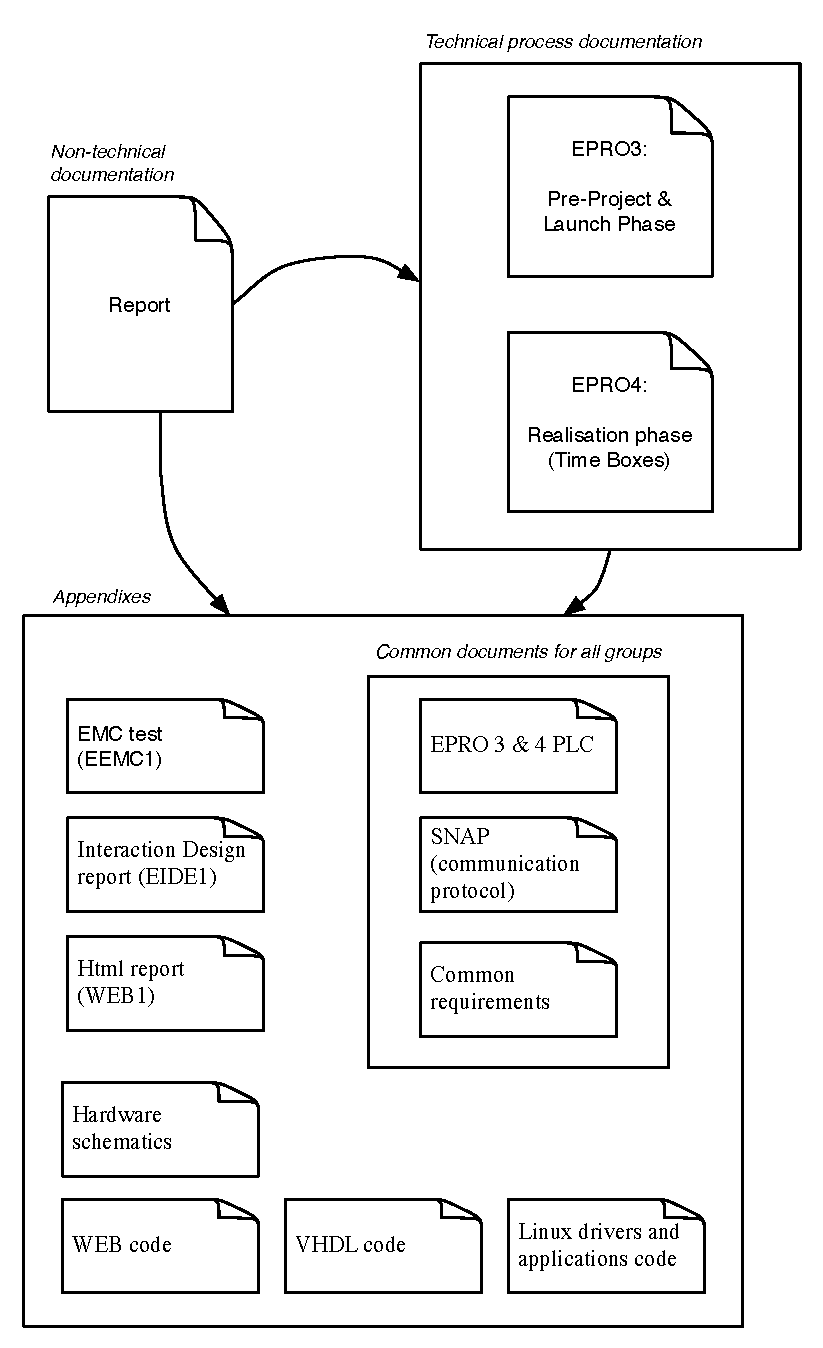
\includegraphics[width=0.5\textwidth]{images/report_ref.pdf}
		\caption*{Project document overview}
	\end{centering}
\end{figure}
This document is divided into three parts. The first part introduce the problem statement. The second part concerns the method that has been used for the working process, and the results for the problem that has been developed through the process. The last part recapitulates the entire project, and verifies if the requirements and the problems, defined in the problem statement are complied with.\\
This document can read from head to tail, without lookup in the process report, for a better understanding of the working process or the technical documentation it is recommended to look up the reference made in the document.\\
Footnotes is assign with at number\footnote{Footnote text here in the bottom of the page} and the text is at the bottom of this page.
\begin{table}[H]
    \begin{tabular}{|l|l|}
        \hline
        \textbf{Abbreviation} & \textbf{Meaning} \\ \hline
        ARM		& Advanced RISC Machine \\ \hline
        BFM		& Bus Functional Module \\ \hline
        EMC		& External Memory Controller* \\ \hline
        EMC		& Electromagnetic Compatibility** \\ \hline
        FPGA	& Field Programmable Gate Array \\ \hline
        PLC		& Power Line Communication \\ \hline
        PS		& Power Switch \\ \hline
        RISC	& Reduced Instruction Set Computing \\
        \hline
    \end{tabular}\\
\textit{* A peripheral in the LPC2478}\\
\textit{** Hardware interference from and with other equipment}\\
\end{table}
%How to read this report (Reading guidelines)
%How was the project initiated?
%What ideas, interests and thoughts are behind your choice of subject?
%Have others worked on the problem and what did they do?
%The introduction may include artefacts from the PreProject, e.g. Rich Picture. It may fill two pages and cover the problem widely
%It may be a good idea to write this part at the end of a project period.